\section{Jonosfärskikten}
\harecsection{\harec{a}{7.3}{7.3}}
\index{jonosfär}
\index{jonosfärsskikt}
\label{vågutbredning_jonosfärskikten}

På höga höjder kan atomer och molekyler färdas långa sträckor utan att
kollidera, de skiktas då genom gravitationens inverkan så att de lättare
atomerna lägger sig över de tyngre.
Kraftig solinstrålning slår loss elektroner från atomerna så att det bildas
positivt laddade atomkärnor och fria elektroner \emph{jonisering}.

Dessa joniserade skikt som delvis består av elektriskt ledande gas har
gett namn åt \emph{jonosfären}.

När en radiovåg passerar genom ett joniserat skikt i atmosfären, kan vågen
ändra riktning, vilket kallas för refraktion.
För att refraktion ska uppstå måste i första hand två villkor uppfyllas, det
första är tillräckligt tät jonisering och det andra är tillräckligt
lång våglängd.
Under ''gynnsamma'' omständigheter kan vågorna till och med böjas av
ner mot jorden, vilket är den viktigaste förutsättningen för långväga
radioförbindelser på kortvåg.

Joniseringen av atmosfären är emellertid oregelbunden och varierar
bland annat med höjden över jordytan, solinstrålning, tidpunkt på dygnet,
årstiden med mera.
Ett antal joniserade skikt kan definieras.
Se bild~\ssaref{fig:bildII7-7}.

\subsection{D-skiktet}
\index{jonosfärsskikt!D-skiktet}
\label{d-skiktet}

\emph{D-skiktet} förekommer under den ljusa delen av dygnet på en höjd av cirka
\SIrange{50}{90}{\kilo\metre}.
På \SIrange{70}{90}{\kilo\metre} höjd orsakas joniseringen huvudsakligen av
röntgenstrålar från solen, medan den kosmiska strålningen har störst påverkan på
\SIrange{50}{70}{\kilo\metre} höjd.
D-skiktet dämpar de infallande radiovågorna, med största verkan i
kortvågsområdets lågfrekventa del och under de ljusaste timmarna under sommaren.
D-skiktet har dålig reflektionsförmåga och verkar hindrande på
långdistansförbindelser.

\subsection{Mögel-Dellinger-effekten}
\index{Mögler-Dellinger-effekten}
\index{jonosfärsskikt!black out}

Strålning från gasutbrott på solytan kan jonisera D-skiktet så kraftigt, att
alla radiovågor med frekvenser över cirka \qty{1}{\mega\hertz} dämpas helt,
detta kallas för \emph{Mögel-Dellinger-effekten}.
Radiotrafik som baseras på vågutbredning via jonosfären är då
omöjlig att genomföra under en tidsrymd av ett antal minuter upp till
flera timmar -- det blir ''black out''.

\subsection{E-skiktet}
\index{jonosfärsskikt!E-skiktet}
\label{e-skiktet}

\emph{E-skiktet} (Kenelly-Heaviside-skiktet) är det lägsta reflekterande
jonosfärskiktet.
Det förekommer på en höjd av cirka \SIrange{90}{140}{\kilo\metre} och är mest
koncentrerat på cirka \qty{110}{\kilo\metre} höjd.
E-skiktet alstras av att ultraviolett strålning joniserar syreatomer.
Skiktet reflekterar vågor bäst i kortvågsområdets lågfrekventa del och är
kraftigast under den ljusa delen av dygnet.
På grund av D-skiktets dämpande verkan under de ljusaste timmarna är E-skiktet
mest användbart under grynings- och skymningstimmarna.

Ett säsongmaximum i reflektionsförmågan inträffar under sommaren.
Förbindelseavstånd på upp till \qty{2000}{\kilo\metre} är möjliga.

\subsection{Sporadiska E-skiktet}
\index{jonosfärsskikt!sporadiska E-skiktet}
\index{sporadiska E-skiktet}
\label{sporadiskt_e}

Den starkare solinstrålningen under sommaren orsakar en kraftigare
jonisering i den lägre jonosfären än under vintern.
Inom E-skiktet bildas då sporadiska tunna molnlika partier med mycket hög
joniseringsgrad och stor reflektionsförmåga, det så kallade \emph{sporadiska
E-skiktet} (\(E_s\)).
Vågutbredningen via \(E_s\) är mycket olika på olika latituder och är bäst
omkring 40:e latituden.
Mycket goda långväga förbindelser kan uppnås.

\mediumfig{images/cropped_pdfs/bild_2_7-07.pdf}{Jonosfärskikten}{fig:bildII7-7}

\subsection{F-skiktet}
\index{jonosfärsskikt!F-skiktet}
\index{F-skiktet}
\index{F1@\(F_1\)}
\index{F2@\(F_2\)}

\emph{F-skiktet} är det högst liggande jonosfärsskiktet.
Det förekommer såväl dag- som nattetid på en höjd av
\SIrange{140}{500}{\kilo\metre}.
Den nedre del av skiktet, \SIrange{140}{200}{\kilo\metre}, uppvisar andra
variationer än den övre delen.
F-skiktet beskrivs därför som två skikt, \(\mathrm{F_1}\) upp till cirka
\qty{200}{\kilo\metre} höjd och \(\mathrm{F_2}\) över denna höjd.

Liksom E-skiktet, påverkas \(\mathrm{F_1}\)-skiktet kraftigt av
instrålningen från solen.
Det når sin högsta joniseringsgrad ungefär en timme efter högsta lokala
solståndet och förekommer endast under sommaren.
Under natten förenar sig \(\mathrm{F_1}\)- och \(\mathrm{F_2}\)-skikten till
ett enda F-skikt.

\(\mathrm{F_2}\)-skiktet är det skikt som varierar mest i tiden och rummet.
Den högsta joniseringsgraden inträffar vanligen sent efter högsta lokala
solståndet, ibland under aftontimmarna.
Skiktets maximala jonisering är på \SIrange{250}{350}{\kilo\metre} höjd på
mellanlatituder och på \SIrange{350}{500}{\kilo\metre} höjd vid ekvatorn.
På mellanlatituder ligger den största elektrontätheten i skiktet högre under
natten än under dagen.
Vid ekvatorn är förhållandet omvänt.

Reflektioner i \(\mathrm{F_2}\)-skiktet möjliggör att stora
avstånd kan överbryggas (1 hopp = \SIrange{3000}{4000}{\kilo\metre}).

\mediumfig{images/cropped_pdfs/bild_2_7-08.pdf}{Jonosfärsutbredning.}{fig:bildII7-8}

\subsection{Höjd till reflekterande skikt}
\index{jonosfärsskikt!höjd till skikt}

När en radiovåg, som riktas rakt uppåt, träffar jonosfären kan den antingen
\begin{itemize}
  \item absorberas -- sugas upp
  \item reflekteras
  \item tränga igenom.
\end{itemize}

Vilket som inträffar beror på den använda frekvensen.
Ju högre frekvensen är på den uppåtriktade radiovågen, desto högre upp i ett
atmosfärskikt kommer avböjningen tillbaka att inträffa.
Höjden till skiktet beräknas ur radiovågens utbredningshastighet och
utbredningstid fram och åter mellan skiktet och jordytan.

\subsection{Kritisk frekvens}
\harecsection{\harec{a}{7.4}{7.4}}
\index{kritisk frekvens}

Vid en viss övre frekvens upphör reflektionen i atmosfärskiktet och
vågen går ut i rymden i stället för ner till jordytan.
Denna frekvens kallas den \emph{kritiska frekvensen}, som varierar med
joniseringsgraden i atmosfären.
Den kritiska frekvensen är högst vid högt solfläckstal, såväl i E- som i
F-skikten, eftersom joniseringsgraden då är störst.
Den kritiska frekvensen för E-skiktet varierar mellan cirka
\SIrange{1}{4}{\mega\hertz} beroende på tidpunkt i solfläckscykeln och tid på
dagen.
Den kritiska frekvensen för F-skiktet varierar med tid på dagen, årstid och
skede i solfläckscykeln.
Den kan variera från \SIrange{2}{3}{\mega\hertz} natten under ett
solfläcksminimum till \SIrange{12}{13}{\mega\hertz} på dagen under ett
solfläcksmaximum.

\subsection{Kritisk vinkel}
\index{kritisk vinkel}

Rymdvågen måste träffa ett joniserat atmosfärskikt med en tillräckligt
flack vinkel för att reflekteras, den så kallade kritiska vinkeln.
Denna vinkel är frekvensberoende.
Allt eftersom den utsända frekvensen ökas ytterligare över den kritiska
frekvensen, måste vågen träffa atmosfärskiktet i en allt flackare vinkel för att
vågen ska reflekteras mot jordytan.
Genom att sända ut vågen i mycket flack vinkel mot \(\mathrm{F_2}\)-skiktet kan
långa distanser överbryggas vid frekvenser som är upp till 3,5 gånger den
kritiska frekvensen.

Så snart den kritiska frekvensen är högre än frekvensområdet för ett
amatörband är det alltså möjligt att kommunicera över rymdvåg på detta band.
Det kan ske över alla avstånd, allt ifrån skipavståndet till det som avgörs av
utbredningsförlusterna.

\subsection{Högsta användbara frekvens (MUF)}
\harecsection{\harec{a}{7.6}{7.6}}
\index{högsta användbara frekvens}
\index{MUF|see {högsta användbara frekvens}}
\index{Maximum Usable Frequency (MUF)|see {högsta användbara frekvens}}

Radiovågorna vandrar från sändaren till en avlägsen mottagare genom att
reflekteras en eller flera gånger i jonosfären och på jordytan.
Se bild~\ssaref{fig:bildII7-8}.
För att detta ska ske kan frekvensen inte vara högre än den
\emph{högsta användbara frekvensen} (eng. \emph{Maximum Usable Frequency, MUF})
för en viss överföringssträcka.

MUF är högst mitt på dagen eller tidig eftermiddag.
Allra högst är MUF under perioder av högt solfläckstal och kan då komma
upp till över \qty{30}{\mega\hertz}.
Under tidiga morgontimmar sjunker MUF ofta under \qty{5}{\mega\hertz} och ibland
ännu lägre särskilt vintertid.

De jonosfäriska förlusterna är lägst nära MUF och ökar snabbt under
dagtid för lägre frekvenser.
Aktuella MUF-data publiceras periodiskt i olika media, men kan också
överslagsberäknas med hjälp av speciella datorprogram.

\subsection{Optimal trafikfrekvens (FOT)}
\index{optimal trafikfrekvens}
\index{FOT}

I praktiken är det av intresse att veta det frekvensområde där
kommunikation bäst kan genomföras.

Rekommenderad övre frekvensgräns för en tillförlitlig radioförbindelse
kallas \emph{optimal traffic frequency (FOT)} och väljs något under
MUF som marginal för oregelbundenheter och turbulens i jonosfären,
liksom för korttidsavvikelser från det förutsagda månatliga
medianvärdet för MUF.
FOT är vanligen ungefär \qty{15}{\percent} lägre än MUF.

\newpage
\subsection{Lägsta användbara frekvens (LUF)}
\index{lägsta användbara frekvens}
\index{LUF}
\index{Lowest Usable Frequency (LUF)}

Ju lägre sändningsfrekvens som väljs, desto mer dämpas vågorna i
jonosfären, intill den frekvens då de inte kan uppfattas.
Den \emph{lägsta användbara frekvensen}
(eng. \emph{Lowest Usable Frequency, LUF}) är den
frekvens som ger tillfredsställande kommunikation för en viss
utbredningsväg och vid en viss tidpunkt.

Vid frekvenser under LUF är mottagning inte möjlig eftersom brusnivån
då är för hög.
Ju mer frekvensen höjs över LUF, desto bättre blir signal-brus-förhållandet.

Till skillnad från MUF, som endast påverkas av de jonosfäriska
förhållandena, kan LUF till en del påverkas genom utsänd effekt och bandbredd.
Generellt kan LUF sänkas cirka \qty{2}{\mega\hertz} för varje
\qty{10}{\decibel} ökning av \erp.

\begin{figure*}[t]
  \begin{center}
    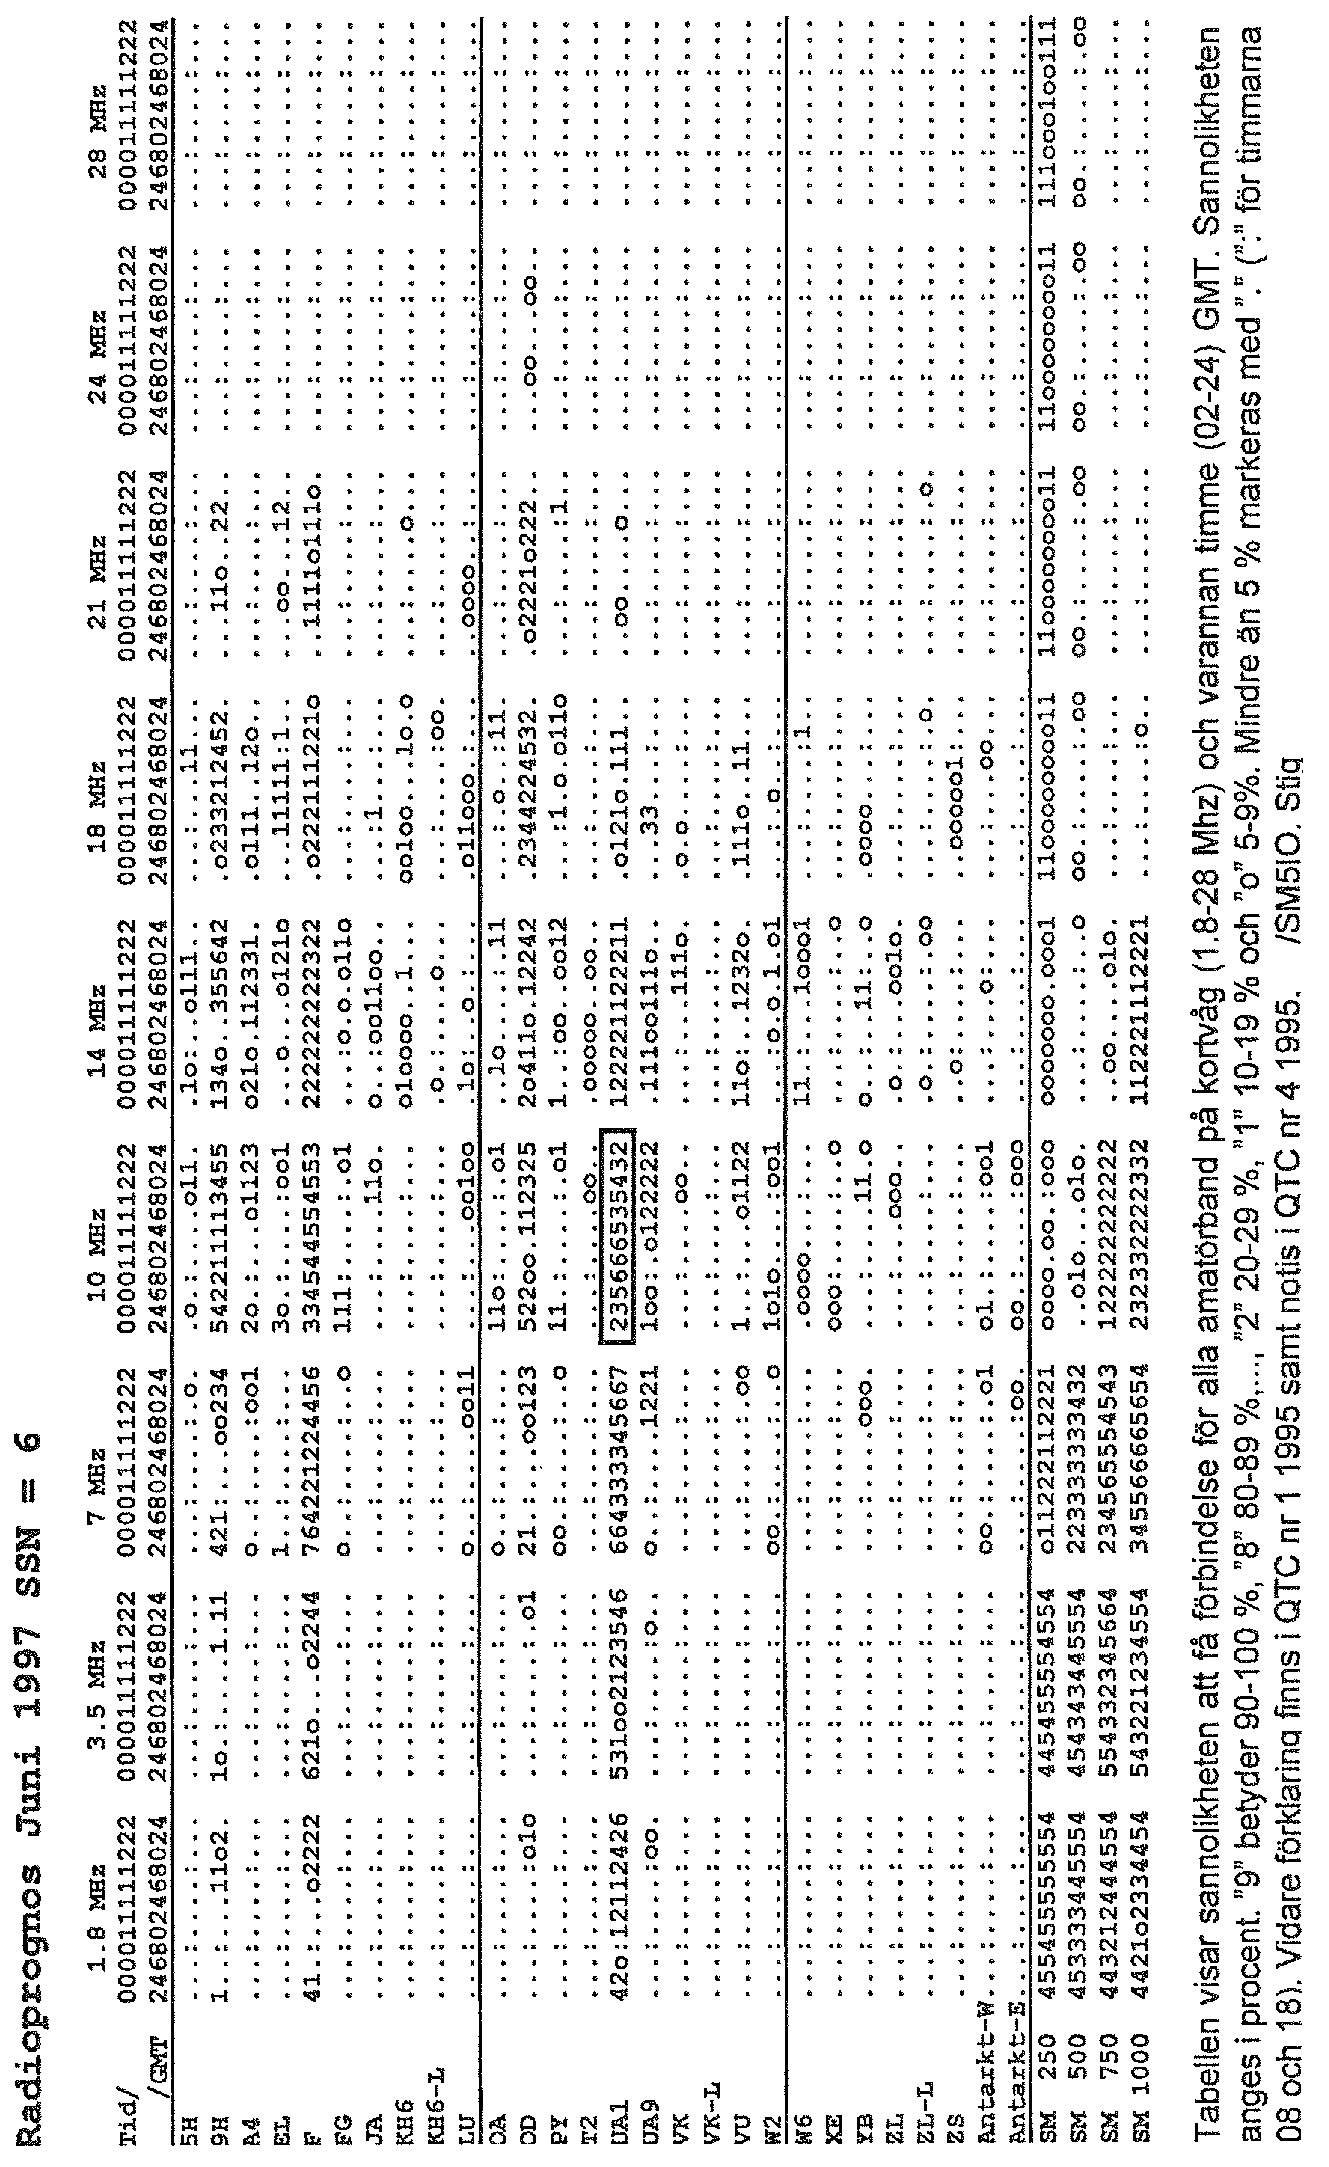
\includegraphics[width=0.6\textwidth,angle=270]{images/cropped_pdfs/bild_2_7-09.pdf}
    \caption{Radioprognos för amatörradiobanden på kortvåg}
    %% k7per: konverted from fig macro?
    %% {fig:bildII7-9}
    \label{fig:bildII7-9}
  \end{center}
\end{figure*}

\subsection{Vågutbredningsprognoser}
\index{vågutbredningsprognoser}
\index{vågutbredning!prognoser}
\index{vågutbredning!propagation forecasts}

Det finns ett brett utbud av datorprogram och webbsidor som ger
vågutbredningsprognoser och observationer som underlättar för att förstå vilka
frekvenser som kan vara aktuella för DX-trafik och när på dygnet som
förhållandena är bäst.
Verktygen är av två typer: långtidsprognoser och ''rymdväderobservationer''.
Verktygen för långtidsprognoser har utvecklats under många decennier för att
till exempel kunna ta fram frekvensscheman för utlandsprogrammen på kortvåg.
Det mest kända verktyget är VOACAP, ursprungligen framtaget för Voice of America
(VOA).
VOACAP har fått ett fantastiskt fint webbgränssnitt för radioamatörer av
Jari/OH6BG.
Verktygen fungerar så att man matar in solaktiviteten och tidpunkten.
Baserat på en medeljonosfär beräknar verktyget en förväntad MUF och signalstyrka
på olika band.
Solaktiviteten uttrycks i form av solfläckstalet (eng. \emph{Sun Spot Number, SSN}).
SSN får man fram genom att observera solen och räkna antalet fläckar.
SSN publiceras på internet dagligen på många olika internetsidor.
Ett annat mått, som är nära korrelerat med solfläckstalet är solflödet (eng.
solar flux) som antingen mäts i \unit{\watt\per\metre\squared} eller med hjälp
av ett index, SFI (eng. \emph{Solar Flux Index}).
Ett SFI på 100 motsvarar en genomsnittlig solaktivitet.

%%\largefig{images/cropped_pdfs/bild_2_7-09.pdf}{Radioprognos för amatörradiobanden på kortvåg}{fig:bildII7-9}
